\documentclass[11pt,a4paper]{article}
\usepackage[margin=24mm]{geometry}
\usepackage{amsmath,booktabs,graphicx,hyperref}
\hypersetup{hidelinks}
\title{One common theory and three complete applications: measured proof costs}
\author{Human Compression project}
\date{11 October 2026}
\begin{document}\maketitle
\noindent The main results of three complete historical manuscripts are recovered by one common proof and three applications. Counting NFC-normalized characters other than whitespace, the source texts total $71{,}375$ and our new complete written proofs total $38{,}568$, giving
\[
 \frac{71{,}375}{38{,}568}=1.850627\ldots .
\]
The full shared theory is charged once within this topic. This is a manuscript-length comparison under the already accepted main-result contracts and a common declared classical background; unmeasured external proofs are not assigned cost zero.

\begin{center}\begin{tabular}{lrrrr}\toprule
Document & Historical & Previous & New & Conditional factor\\\midrule
Shared theory & --- & 18,264 & 19,362 & ---\\
L083 / PSL polytopes & 20,885 & 8,213 & 2,914 & 7.167\\
L079 / PGL polytopes & 20,908 & 5,737 & 1,851 & 11.296\\
L021 / PSL maniplexes & 29,582 & 21,681 & 14,441 & 2.048\\\midrule
Complete written total & 71,375 & 53,895 & 38,568 & ---\\\bottomrule
\end{tabular}\end{center}
Each conditional factor divides the complete source manuscript by its application after acquiring the common theory and required finite program. The shared acquisition costs $19{,}362+7{,}565$ characters and is charged once in the complete topic.

The sources are Leemans--Schulte's \emph{Groups of type $L_2(q)$ acting on polytopes} and \emph{Polytopes with groups of type $PGL_2(q)$}, and Leemans--Toledo's \emph{Maniplexes with automorphism group $PSL(2,q)$}. Exact author editions and all result qualifications remain bound in the protocol. In particular, L079's semilinear census and conjecture, and L021's final PGL question, are outside these recovered main results, although their source text is counted. The existing L021 corrections are preserved.

The mathematical change is a common theorem for four distinct string involutions with proper $S_4/A_5$ ends and odd outer labels. It derives the three exact marked groups, their intersection property and uniqueness. The projective restriction, finite calculation, geometry and extension for full or maximal end groups are proved once. The applications supply their field identifications and, for L021, the proofs for every prime in its stated families and the source marking. The underlying local classes and universal table are historical results. No historical novelty or additional question credit is asserted.

The previous complete written proof has $53{,}895$ characters. The new proof removes $15{,}327$ of them while its shared theory grows by $1{,}098$ characters. This comparison records complete arguments, not a count of theorem boxes or a forecast of a future library.

\newpage
\noindent\textbf{Required computation and diagnostics.}
The complete merged finite program contributes $7{,}565$ characters, including every literal correction witness. Adding the complete diagnostic program contributes another $5{,}173$. Consequently
\begin{align*}
 \frac{\text{source text}}{\text{new proof + required program}}
 &=\frac{71{,}375}{46{,}133}=1.547157\ldots,\\
 \frac{\text{source text}}{\text{new proof + required program + diagnostics}}
 &=\frac{71{,}375}{51{,}306}=1.391163\ldots.
\end{align*}
These are comparisons using known costs: historical program costs and the full cost of retained classical proofs are unknown. Required plus diagnostic code totals $12{,}738$, compared with $12{,}599$ for all old programs. Thus the gain including diagnostics does not come from deleting diagnostic costs. Available partial Lean certificates are inventoried separately; their presence is not a full formal proof of the classification, and full formalization cost is unknown.

\begin{center}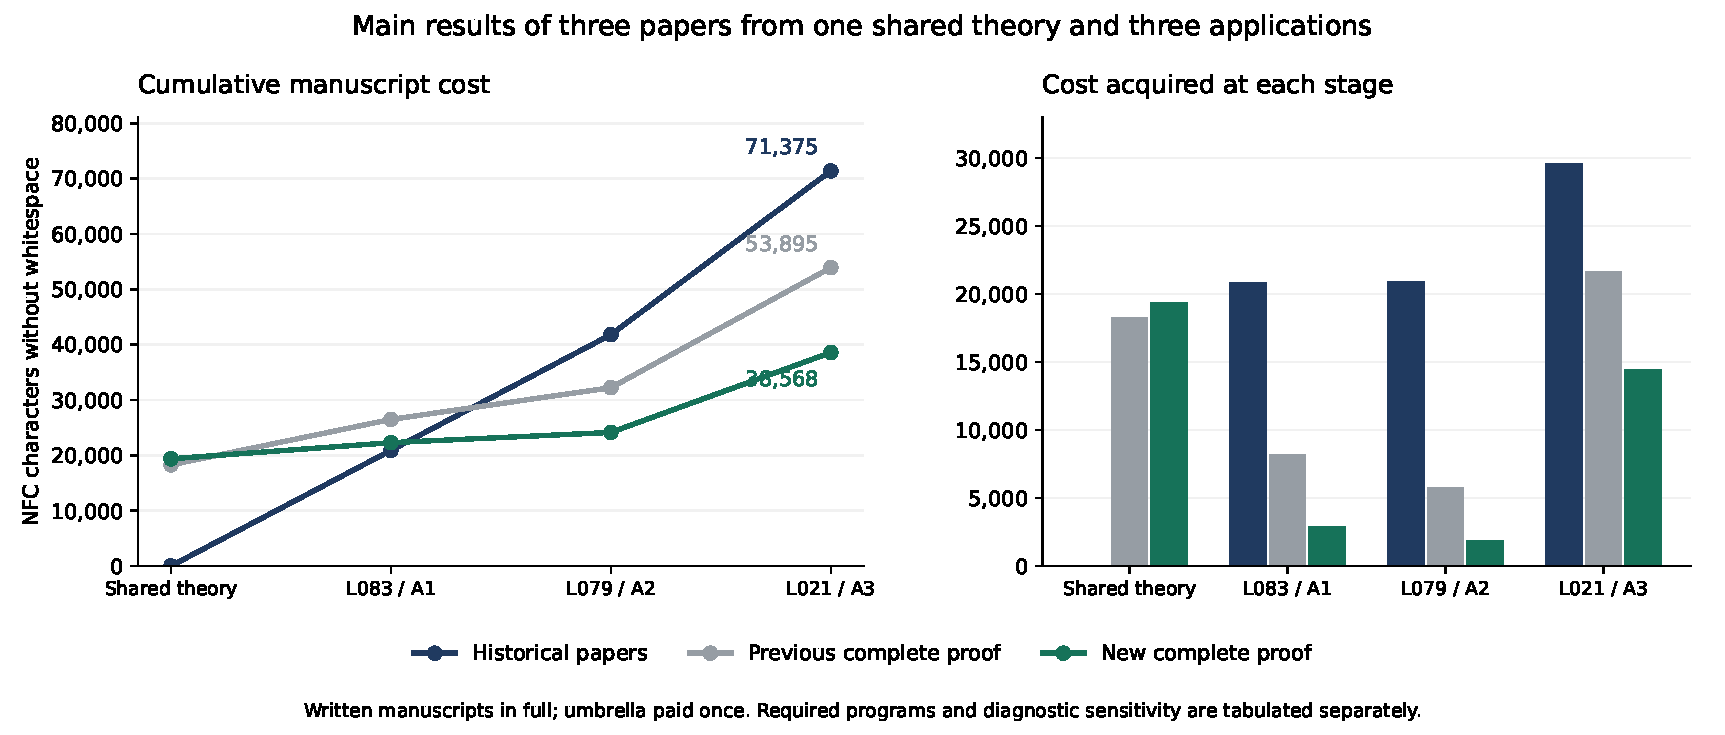
\includegraphics[width=\textwidth]{costs.pdf}\end{center}
The acquisition stage pays the full shared manuscript. Application stages then pay the complete local papers. The displayed curve is a declared accounting order, not a reconstruction of historical discovery or evidence of a repeated sawtooth. The machine-readable CSV also contains complete cumulative costs including programs. The merged required program is paid once at acquisition; earlier A3 programs were attached to its application, so intermediate program curves reflect that packaging convention.

All fifteen documents were independently recounted in all ten NFC/NFKC metric coordinates, giving 150 exact matches. The old and new complete rules selecting text coincide; only individually bound repeated page furniture is removed. Eight parentheses around source matrices extract incorrectly; individually checked substitutions preserve their lengths. Eight negative controls reject altered inputs, boundaries and scope. The finite proof passed an independent fresh replay with five semantic mutations rejected.
\end{document}
